% do not change these two lines (this is a hard requirement
% there is one exception: you might replace oneside by twoside in case you deliver 
% the printed version in the accordant format
\documentclass[11pt,titlepage,oneside,openany]{book}
\usepackage{times}
\usepackage{caption}
\usepackage{longtable}
\usepackage{pgfplots}
\pgfplotsset{width=11.5cm,compat=1.9}

\usepackage{graphicx}
\usepackage{latexsym}
\usepackage{amsmath}
\usepackage{amssymb}
\usepackage{glossaries}
\usepackage{lscape}
\usepackage{ntheorem}
%\usepackage[table,xcdraw]{xcolor}
% \usepackage{paralist}
\usepackage{tabularx}

% this packages are useful for nice algorithms
\usepackage{algorithm}
\usepackage{algorithmic}

% well, when your work is concerned with definitions, proposition and so on, we suggest this
% feel free to add Corrolary, Theorem or whatever you need
\newtheorem{definition}{Definition}
\newtheorem{proposition}{Proposition}


% its always useful to have some shortcuts (some are specific for algorithms
% if you do not like your formatting you can change it here (instead of scanning through the whole text)
\renewcommand{\algorithmiccomment}[1]{\ensuremath{\rhd} \textit{#1}}
\def\MYCALL#1#2{{\small\textsc{#1}}(\textup{#2})}
\def\MYSET#1{\scshape{#1}}
\def\MYAND{\textbf{ and }}
\def\MYOR{\textbf{ or }}
\def\MYNOT{\textbf{ not }}
\def\MYTHROW{\textbf{ throw }}
\def\MYBREAK{\textbf{break }}
\def\MYEXCEPT#1{\scshape{#1}}
\def\MYTO{\textbf{ to }}
\def\MYNIL{\textsc{Nil}}
\def\MYUNKNOWN{ unknown }
% simple stuff (not all of this is used in this examples thesis
\def\INT{{\mathcal I}} % interpretation
\def\ONT{{\mathcal O}} % ontology
\def\SEM{{\mathcal S}} % alignment semantic
\def\ALI{{\mathcal A}} % alignment
\def\USE{{\mathcal U}} % set of unsatisfiable entities
\def\CON{{\mathcal C}} % conflict set
\def\DIA{\Delta} % diagnosis
% mups and mips
\def\MUP{{\mathcal M}} % ontology
\def\MIP{{\mathcal M}} % ontology
% distributed and local entities
\newcommand{\cc}[2]{\mathit{#1}\hspace{-1pt} \# \hspace{-1pt} \mathit{#2}}
\newcommand{\cx}[1]{\mathit{#1}}
% complex stuff
\def\MER#1#2#3#4{#1 \cup_{#3}^{#2} #4} % merged ontology
\def\MUPALL#1#2#3#4#5{\textit{MUPS}_{#1}\left(#2, #3, #4, #5\right)} % the set of all mups for some concept
\def\MIPALL#1#2{\textit{MIPS}_{#1}\left(#2\right)} % the set of all mips

\makeglossaries

\newglossaryentry{cs}{%
name={cs},%
description={Customer Satisfaction}%
}



\begin{document}

\pagenumbering{roman}
% lets go for the title page, something like this should be okay
\begin{titlepage}
	\vspace*{2cm}
  \begin{center}
   {\Large Capitalism X\\}
   \vspace{2cm} 
   {Handbook \& Documentation\\}
   \vspace{2cm}
   {presented by\\
   Philipp Epstein \\
    Daniel G\"otz \\
Maike Jansen \\
Nike Klaubert \\
Salih \"Ozdemir \\
Livja Papuciu \\
Janine Salomon \\
Steffen Waldmann \\
   }
   \vspace{1cm} 
   {submitted to the\\
    Data and Web Science Group\\
    Prof.\ Dr.\ Heiner Stuckenschmidt\\
    University of Mannheim\\} \vspace{2cm}
   {March 2019}
  \end{center}
\end{titlepage} 

% no lets make some add some table of contents
\tableofcontents
\newpage

\listoffigures

\listoftables
\printglossary[style=long]
% evntuelly you might add something like this
% \listtheorems{definition}
% \listtheorems{proposition}

\newpage
% okay, start new numbering ... here is where it really starts
\pagenumbering{arabic}

\chapter{From a small startup to a global enterprise}
\label{cha:intro}
\section{What to expect from Capitalism X (CapX)}
Nike\\
Business simulation games...Fancy introduction, Target audience\\
Goal of business simulation game\\
User skills? Thinking economic entrepreneurial spirit...\\

Did you ever tested out your economic skills and entrepreneurial spirit? Did you ever wish to take action and do things your way? Did you ever thought that with the steering wheel in your hand, you'd give a company a whole new direction and possibility to rise? \\
CapitalismX now gives you the possibility to become CEO! This business simulation game, which is equally fun and educative, gives you the chance to prove your successful way of managing a company through decades.\\

\emph{Very Important:} Besides being a game-play handbook, this document also addresses the game mechanisms working in the background
 
\section{Player's role}
Maike\\
The user assumes the role of CEO for either a start-up or a midsize company which is about to fail. During his career, the player encounters several obstacles and leads the business. So, the user slips into various roles, such as head of human resources, production or logistics, in order to take the necessary measures to run a successful business. Daily tasks include hiring, firing, motivating and training employees, innovating and manufacturing products, deciding on the product portfolio, dealing with government issues and taking financial figures into account.
In summary, the player decides on all the features provided in our game. These decisions are included in finance, human resources, procurement, production, warehouse, logistics and marketing and affect the performance of the company.

\section{Setting \& Story}
\label{SettingStory}
Maike\\
Timeframe from 1990 to 2017 in the first phase, Progress\\
The setting of the game is a fictional map of a town/city.  The player has to choose where to set up his first shop, in a vacant distant area or downtown.\\
Functional\ Non-functional buildings\\
Functional buildings: bank, government building, consultant firm, harbor(import/export), marketing firm, competitors \\
Non-functional buildings: City centre, Parks(increase employee satisfaction), sea/ river, roads(transportation)\\
Own currency: capcoins cc (value comparable to US Dollars) \\
Democratic government \\
One day in the game is 3 seconds in real time\\
Total playtime: 15 hours.\\
Storyline:\\
Mid-size IT company\\
Start option 1: We buy a mid size IT company which is about to fail 
(bad management)\\
Start option 2: We found a new Start-Up, so we can choose our employees and products ourselves
Different starting capitals\\
Products: see Product Flow Charts\\
Trading components\\
Make or Buy decisions for some products, not components\\
Organize your entire company from the CEO's perspective (incl. HR, Finance, Manufacturing, ect.)\\
Customer simulation regarding services, support and products \\
External events:\\
Handle random events(e.g natural disasters) (defined in Problem-Influence-Matrix)\\
And handle events that will be triggered by game settings(fire-old machines, company shut down - low eco-index,etc... )\\
Integration of games within CapX, e.g. play a round of Tetris to clean up the mess  in your warehouse (put in Outlook?)\\


\chapter{How to play CapX}
\label{cha:theory}
 This chapter deals with the interface, options, content of the game

\section{Getting started with CapX}
Steffen, Nike
Halbe Seite\\

\label{sec:prelim}
Starting screen selections, first steps
\begin{definition}
\label{def:evil}
An entity is evil if it is not a good entity.
\end{definition}

Did you ever tested out your economic skills and entrepreneurial spirit? Did you ever wish to take action and do things your way? Did you ever thought that with the steering wheel in your hand, you'd give a company a whole new direction and possibility to rise? \\
CapitalismX now gives you the possibility to become CEO! This business simulation game, which is equally fun and educative, gives you the chance to prove your successful way of managing a company through decades.\\


\section{Interface \& Features}
\label{sec:good}

\subsection{Controls}  
Nike and Salih
War Room and what to choose? How does everything look like, which buttons etc. pause button / fast-forward button???\\
\subsection{Financials}
Nike, Salih\\
Internal and external financing vs. equity and debt financing\\ short theoretic description, but not all is relevant in our game. \\

Financials occur throughout the whole company as it can be seen as the engine that keeps the whole company running. The entry point for the financial actions is the finance dashboard. You may find it by clicking on the finance button [screenshot] from the navigation bar at the top left. The dashboard gives you a detailed overview about several areas at first glance:

\begin{itemize}
    \item Cashflow, which is basically your profit and loss statement displaying revenues, expenses, and profit on a quarterly basis.
    \item Statistics, showing the development of salaries and total sales in visualized graphs.
    \item Company information, divided into cash, assets, liabilities and company net worth. This view gives you information about the current liquidity of your company.
    \item Bank, providing the possibility to request a loan from the bank or to get an overview about current loans.
    \item Investments, where the you might invest some money in the stock market.
    \item Product performance, giving an overview about product specific key performance indicators, such as the sum of material costs per product.
\end{itemize}

The cashflow, statistics, company information and product performance are solely descriptive information, that is generated from the actual settings defined by you as the player or by your company’s performance. The goal of these areas is to provide an overview about the general financial performance status of the company and should give you hints about adapting some parameters. \\
The bank and the investment areas need input from your side. To start with the bank, [SALIHs STUFF].\\
basic Idea: Player asks for a loan \& gets 2-3 offers with different loan types. 
\begin{itemize}
    \item short term: 1-12 months (interest rate 6-18\%)
    \item midterm: 1-5 years (interest rate 3-6\%)
    \item Long term greater than 5 years (1.85-2\%)
\end{itemize}
Player always receives an offer from the bank matching the business situation (more precisely in the Game Mechanism). The receives an offer for the 01th of the following month with fixed amount, fixed interest rate, fixed retirement, fixed term.
The player has the choice of accepting or rejecting the offer.\\

Apart from that, you might invest some money into innovations on the stock market, which is similar to the well known DAX stock market. As this may be a risky undertaking, due to the regular oscillations on this market, a good idea is to spend only a reasonable amount of money there. \\
%\subsection{Investments}
\label{sec:investments_simulation}

 Investments in CapitalismX are a way to allocate your residual cash to assets with an expected profit. However, each investment is risky and positive return isn't guaranteed. Thus, your liquidity may suffer if you put too much money into investments.
  
  We decided for three classes of investments with different expected returns and assume higher risk for higher return:
\begin{itemize}
	\item Real estate fund
	\item Stocks (index fund)
	\item Venture capital fund
\end{itemize}

Although return distributions are negatively skewed and characterized by an excess kurtosis \cite{ANDERSEN200143}, a normal distribution can be used as an approximation \cite{doi:10.1080/01621459.1972.10481297}. In 2017, the expected return for real estate in the US is about $7\%$ \footnote{https://www.msci.com/documents/10199/f3d1af7c-6069-6e60-a818-71ca9c45e85c}. The compounded annual return of the S\&P from its introduction in 1965 to 2017 is approximately $10\%$ \footnote{http://www.berkshirehathaway.com/letters/2017ltr.pdf}. Venture capital funds in the US have an expected return of $14.2\%$ \footnote{http://www.eif.org/news\_centre/publications/eif\_wp\_41.pdf}.

In our game, the investment worth adjusts daily. Therefore, we take the geometric mean of the average yearly return $\overline{\mu_y}$ to estimate the expected daily return:
\begin{equation}
	\overline{\mu_d} = \sqrt[365]{\frac{1 + \overline{\mu_y}}{1}}
\end{equation}

For our game, we use the return volatility as a representative of the risk of an investment. In an efficient market, a higher risk has to correspond to a higher return. As we are not able to model more complex anomalies like volatility clustering \cite{lux2000volatility} we choose the daily standard deviation $\sigma$ by testing different values instead of relying on historical data in order to allow reasonable game mechanics. However, as a reference point, the yearly standard deviation of the S\&P 500 was 19.7\% \footnote{https://seekingalpha.com/instablog/605212-robert-allan-schwartz/4831186-annual-returns-s-and-p-500-1928-2015}. For our game, we choose the yearly standard deviations 0.2, 0.3 and 0.5 for real estate, stocks and venture capital respectively.
As we specify the yearly standard deviation $\sigma_T$. Thus, we need to calculate the standard deviation of a single day, which we assume is the same in each period. \textit{square-root-of-time-rule} gives the standard deviation of the entire time frame $T$.
\begin{equation}
    \sigma_T = \sigma*\sqrt{T}
\end{equation}
Thus, we can calculate the daily return from the yearly returns by applying algebraic transformations:
\begin{equation}
    \sigma = \frac{\sigma_T}{\sqrt{T}}
\end{equation}
In the end, our daily return is generated by a Gaussian distribution:
\begin{equation}
	\mu_d \sim \mathcal{N}(\overline{\mu_d},\,\sigma^{2})\,.
\end{equation}

Pricing and selling of goods might appear as a financial task to you, but in fact, you will find information about these topics in the manufacturing view.\\ 

%Pricing and selling -- put into production view \\
%pricing: user sees cumulated costs per product incl. employee costs (LIVJAS formel) and may decide on a profit margin to add to the costs. He gets some hints and the value addded as percent. (explain UI part in 4.x chapter).

\subsection{HR}
Maike and Philipp \\
Fundamentals of HR: the vision / mission, the corporate policy and the sustainability of a company.\\
Individual components contained in an HR process:
This includes personnel planning, recruitment, compensation and benefits, training and development and performance management.\\
Personnel planning contains the determination of employee requirements, including number (capacity per head), quality, time/duration, location (domestic/foreign, location, department, cost center) and costs. Steps of recruitment are needs assessment, advertising, selection, negotiation and introduction / training. The aim is to achieve a cost-effective and fast procurement of the desired employees. This involves identifying, interviewing and hiring high-performing employees and is essential for long-term success. In addition, guidelines and procedures must be established for the hiring and recruitment process. Compensation and benefits means creating, managing and improving a company's compensation and performance structures. Wages and benefits are two crucial factors that ultimately determine how well your employees feel about your company and how likely they are to stay with it in the future. Therefore, a company must develop an effective compensation system. Training and development includes the ability to create training programs that solve the performance problems of employees and create additional incentives for employees to improve further and thus also advance the company. Thereby, employee feedback is necessary to continuously improve the quality of a company's training programs. Furthermore, the development and implementation of a complete performance management and improvement process is an essential capability of a company. The design of the performance assessment process, its maintenance and the effective monitoring of its implementation represent challenging tasks for a company.
\\
How are all these components considered in our game? What is the goal of the player from the HR point of view?

\subsection{Production}
Livja, (Nike for Pricing and Selling) \\
 production is composed of three main elements: procurement(harbour), manufacturing, logistics(relate to following paragraph)\\
explain each sub-unit of these elements and adapt explanation and functions to the mock-up
procurement of products - component, component level, units, price, supplier \\
manufacturing
\begin{itemize} 
\item production technology-explain range of measurement, graph, possibilities to purchase machinery
\item manage individual machines (maintain, upgrade, sell) how these actions affect budget and technology measures
\item overall status of the machinery in the plant
\item production performance(production technology+employee skills)graph, how much each of these factors affect the overall production performance
 \item possible investments- player can decide how to improve production performance based on these options, can also decide the amount of Cap-Coins(cc) to invest
 \begin{itemize} 
 \item R\&D
 \item System Security
 \item Automation
 \end{itemize}
 \item eco-index(explain range)- how eco-index deteriorates, improves, events that may be triggered that require government intervention
\end{itemize}

\subsubsection{Procurement}
Nike explain how to use the procurement part.

\subsection{Marketing}
Janine\\
manage internal communication, external communication and legal topics for your company 
\\
internal communication: 
\begin{itemize} 
\item offering online courses and see an overview of the courses offered the last two years. (go green, stress management, teamwork, diversity, ...) 
\item perform an employee survey to get information about the employee satisfaction overall and in the single departments
\item perform an employee survey to see in detail what needs to be improved to achieve a higher employee satisfaction. See statistics of the last three employee surveys. (more internal courses, higher boni, more flexible working times, better work conditions, more training, other factors that play a role in calculating the employee satisfaction)   
\end{itemize}
external communication: 
\begin{itemize} 
\item Mange campaigns and  have an overview of the campaigns performed during the past two years.
Green company, diversity, CSR, promoting company, refugee program, etc. 
\item make official statements for the company to mitigate negative impacts. (data privacy and security efforts, stable prices, safe delivery times, apologize for longer delivery times, ...) 
\item market research 
\begin{itemize} 
\item Conduct market research to get useful information about your products, prices and general market position.
You are able to do the market research by yourself (in house) or  hire a market research institution (external). The advantage of doing the research in-house is the lower price. For every internal research you can choose between a verbal, telephone, written or online survey. It is important to understand the pros and cons of each type. For example, an oral survey is more expensive than an online one, but yields immediate results. By contrast, an online survey takes longer, which can cause the data to be slightly out of date. 
A detailed list of the pros and cons can be found in the table below. (insert table -todo) 
\item See the results of your research performed during the last two years 
\begin{itemize} 
\item price sensitive research for a specific product
\begin{itemize} 
\item Provides a price sensitive analysis for a specific product
\item The study isolates the impact of the price on the market shares while holding all the other factors (quality, …) constant.
\item The research shows the results for 9 price levels around the reference price (input), the price levels are from -20\% to +20\% in 5\% steps 
\item add example report -todo
\end{itemize}
\item customer satisfaction (company at all, specific product / last year in quarters) 
\begin{itemize} 
\item provides customer satisfaction estimated for a specific product (input) or the company at all
\item shows the results for the last four quarters 
\item add example report -todo
\end{itemize}
\item market statistic (overall company, product level) 
\begin{itemize} 
\item provides a variety of market information 
\item add example report -todo
\end{itemize}
\end{itemize}
\end{itemize}
\end{itemize}
legal topics: 
\begin{itemize} 
\item Lobbying (lobbyists can be used to influence the government and thereby mitigate the impact of e.g. environmental regulations on the company)
\item hire management consultancy (can help you to make important decisions and uncover mistakes that happen in your company) 
\end{itemize}

\subsection{Logistics}
Janine
\begin{itemize} 
\item products are sold directly out of the warehouse (all produced products go into the warehouse first) 
\item If the demand for products is higher than the inventory, all products are sold from the warehouse. That means the inventory represents the maximum sales quantity for a product
\item If the demand for a product is lower than the inventory, only the demanded quantity is sold and thus delivered. The remaining products stay in the warehouse and cause storage costs
\item The capacity of the logistics fleet is measured by the number of trucks. Each truck makes it possible to deliver 1000 packages per day.
\item Cost Trucks:
\begin{itemize}
\item cost per delivery of 1000 packages
\item Acquisition costs for the truck (one time)
\item Maintenance costs for the truck (yearly or monthly)
\item trucks can be sold if they are not needed anymore. They are linear depreciated over 9 Years  
\end{itemize}
\item Is the demand and also the inventory of the products higher than the deliver capacity of the trucks and the company has no external logistic partner, the company has to pay a fix deliver price for each package
\item External logistic partner:
\begin{itemize}
    \item can be hired in the job market
    \item have a quality, eco and reliability -index
    \item cost per delivery of one package
    \item contractually agreed fixed costs (yearly or monthly) 
    \item possible to fire the actual partner and hire a new one. Only one logistic partner at the same time possible 
\end{itemize}
\end{itemize}

\section{Build up an empire business}
Janine
\label{sec:business}
https://www.youtube.com/watch?v=NisCkxU544c
\subsection{Choose the portfolio}
Nike \\
Description of products \\
As mentioned above in chapter xxxx, the player may offer two different types of products. Those two different groups are first manufactured goods, and second, retail products that are simply bought as a whole and resold under the company brand \\

To start with the retail products, consisting of two different sub-groups of products: the mass storage devices and the movie playback devices. As the products evolve over the time frame of the game, the scope of the single product group also changes. \\
Mass storage devices will evolve, given a decent investment to innovate, from CD over DVD to BlueRay, from small SD cards to SD cards with very large memory, and from USB Sticks with small memory and in simple versions to evolved versions with large memory. FURTHER DESCRIPTION OF PRODUCTS NEEDED?!
Movie playback devices may evolve from simple video recorders for recording tapes to DVD and BlueRay player, that even can become smart. \\

The larger part of the product portfolio is displayed by the manufactured goods. To produce those, the player has to slip into the role of a strategic head of manufacturing and has to take care about the education and satisfaction of employees in order to provide a high manufacturing and therefore also high product quality; about the procurement of components and warehousing of products; and so on.
The manufactured goods are divided into four product sub-groups, which are notebooks, phones, gameboys, and televisions. \\
Contrary to retail products, the manufactured products consist of single components, that the player needs to buy at the procurement (???) harbour. Also, the player needs engineers in order to aggregate the components to products. As described in section XXXX, the education and skills of the engineers influence the quality of the product. Other than that, the product quality is also determined on the component's actuality. Another difference to the retail products is, that the manufactured product's evolution is depicted by different levels, meaning that a notebook always stays a notebook, but it surely evolves to a higher performing version. To put it into a nutshell, the player has to continuously innovate and invest in new components, skilled engineers, and procurement of components in order to achieve the best competitive products. \\

Apart from that, the player has the possibility to produce more than one product from a product sub-group, which offers various strategic advantages. For example, it is possible to produce two different phones at the same time, to test out different features and product strategies in the market. Phone A could be a very basic, simple phone, suitable for basic tasks like phone calls, messages, emails, surfing in the web. Obviously, Phone A would have a rather cheap price, but also the components do not need to be the latest state of the art tech. Phone B on the other side, could be a very advanced hence expensive phone, including a high resolution camera, high-speed internet connectivity and a fast CPU.\\

\subsection{Lead the right employees}
Janine
\begin{itemize}
    \item find the right mix of employees in the market 
    \item each possible employee has an education level (worker to expert), the initial skill level of the employee is based on the education level
    \item the salary for a employee is affected by there individual skill level.
    \item You can influence the skill level of your employees with trainings 
    \item the higher the skill levels of the employees in the single departments the better the employees are working (e.g. quality in production, support, ...) 
    \begin{itemize}
    \item Trainings are performed on employee level, you decide which employees should be trained 
    \item Costs of training are calculated based on the type of training and the number of employees who are trained
    \item not every training influences the skill level in the same way 
    \end{itemize}
    \item it is also important to build a good work environment for the employees. This can be done by e.g. boni, home office, ...
\end{itemize}

\subsection{Make your company grow}
\begin{itemize}
    \item what are important KPIs
    \item possible way to lead the company
\end{itemize}
how to play your game successfully


\section{Challenges \& Opportunities}
Daniel \\
Planning is important but, but not everything can be foreseen 
Explain real-world background
External factors play a role in real life
Influence on the business, but can nonly rarely be influenced vice versa
Support
Why does events happen, in which areas, --> interface?! pop-up?

\label{sec:evil}

\chapter{Approach to the topic}
\section{Project management}
Nike, Maike, Philipp \\
Timeline, iterative, agile working, feedback loops, project charters, meeting minutes, idea list and capx lingo, google drive, slack and trello blah... 
\section{Way of Working}
What to be confronted with - ralle ich nicht... whut?

\chapter{Game Mechanics and Prototype}
\label{cha:alg}
Game Mechanics were tested via prototype
Technical description of the game, the backend

\section{Finance Simulation}
\label{sec:diag}
Nike, Salih\\
The finance simulation is connecting (?) all other simulations, as costs and profits are ruling an enterprise's daily work. All costs, be it employee costs or costs for training from HR, or manufacturing costs, are collected and subtracted from the profit. On the other side, revenues from either goods sold, machinery sold or shares (?) are added to the profit. Model: simple calculation with adding incoming revenues and substracting costs. Profit is directly mapped to the companies net worth - TAXES????????
\\
graph (differentiate between price and cost, variable vs fixed costs, different sources (e.g. from HR, manufacturing...), financial calculation, kpis (TO DO)\\
Banking system\\
to start manufacturing, player must probably loan money from the bank. Given is xxxx Cap Coins equity capital. The bank has some constraints for giving out loans. The loan must not be larger than 30 percent of the company value, which is for reasons of simplification the current profit. Of course, before manufacturing there is no profit yet, so the first loan is based on the equity capital.\\
If the requested loan is larger than the bank's constraints, the loan is rejected and a personalized offer is provided. In this case, the player can either accept the personalized offer or enter a new loan amount.\\
The bank offers different loan models with varying interests.\\ 
interfaces to all other departments / simulations?\\
initial prices plus cost function for components for single component - basis for manufacturing. in form of data table, based on free imagination.\\
Describe UI \\
Describe how implemented in prototype: net worth of company equals profit, taxes are not considered - profit equals ebit, so interests and taxes are substracted to get net worth\\
PRICING - above in finance section! how is the function displayed in simulation  \\
SELLING - above in finance setion!  how does it influence the revenue\\

\subsection{Investments}
\label{sec:investments_simulation}

 Investments in CapitalismX are a way to allocate your residual cash to assets with an expected profit. However, each investment is risky and positive return isn't guaranteed. Thus, your liquidity may suffer if you put too much money into investments.
  
  We decided for three classes of investments with different expected returns and assume higher risk for higher return:
\begin{itemize}
	\item Real estate fund
	\item Stocks (index fund)
	\item Venture capital fund
\end{itemize}

Although return distributions are negatively skewed and characterized by an excess kurtosis \cite{ANDERSEN200143}, a normal distribution can be used as an approximation \cite{doi:10.1080/01621459.1972.10481297}. In 2017, the expected return for real estate in the US is about $7\%$ \footnote{https://www.msci.com/documents/10199/f3d1af7c-6069-6e60-a818-71ca9c45e85c}. The compounded annual return of the S\&P from its introduction in 1965 to 2017 is approximately $10\%$ \footnote{http://www.berkshirehathaway.com/letters/2017ltr.pdf}. Venture capital funds in the US have an expected return of $14.2\%$ \footnote{http://www.eif.org/news\_centre/publications/eif\_wp\_41.pdf}.

In our game, the investment worth adjusts daily. Therefore, we take the geometric mean of the average yearly return $\overline{\mu_y}$ to estimate the expected daily return:
\begin{equation}
	\overline{\mu_d} = \sqrt[365]{\frac{1 + \overline{\mu_y}}{1}}
\end{equation}

For our game, we use the return volatility as a representative of the risk of an investment. In an efficient market, a higher risk has to correspond to a higher return. As we are not able to model more complex anomalies like volatility clustering \cite{lux2000volatility} we choose the daily standard deviation $\sigma$ by testing different values instead of relying on historical data in order to allow reasonable game mechanics. However, as a reference point, the yearly standard deviation of the S\&P 500 was 19.7\% \footnote{https://seekingalpha.com/instablog/605212-robert-allan-schwartz/4831186-annual-returns-s-and-p-500-1928-2015}. For our game, we choose the yearly standard deviations 0.2, 0.3 and 0.5 for real estate, stocks and venture capital respectively.
As we specify the yearly standard deviation $\sigma_T$. Thus, we need to calculate the standard deviation of a single day, which we assume is the same in each period. \textit{square-root-of-time-rule} gives the standard deviation of the entire time frame $T$.
\begin{equation}
    \sigma_T = \sigma*\sqrt{T}
\end{equation}
Thus, we can calculate the daily return from the yearly returns by applying algebraic transformations:
\begin{equation}
    \sigma = \frac{\sigma_T}{\sqrt{T}}
\end{equation}
In the end, our daily return is generated by a Gaussian distribution:
\begin{equation}
	\mu_d \sim \mathcal{N}(\overline{\mu_d},\,\sigma^{2})\,.
\end{equation}

\section{HR Simulation}
\label{sec:HRsim}
The HR simulation handles all parts of the Human Resources Process. Two employee types have to be hired: Enigneers and Salespeople. The role of HR, Finance and Marketing is performed by the player itself, thus it is not required to hire employees in these departments for the simulation. 

\subsection{Hiring / Firing}
The HR process starts with hiring human resources. Therefore, available engineers and salespeople need to be chosen from the market. Each employee has a requested salary. Moreover, hiring and also firing of employees is associated with cost of 5000 CapCoins. \cite{recruiterbox}

\subsection{Salary}
Salaries are an important factor in the HR process. In order to make the simulation as realistic as possible, we use the following salaries which are derived from a salary-list of a real world IT company. The salaries of available employees are randomized value out of the corresponding salary-range entry in table \ref{tab:Salaries}

\begin{table}
    \centering
\begin{tabular}{c|c}
    \hline
     \textbf{Skilllevel} & \textbf{Salary-range in thousands CC} \\
     \hline \hline
     0-20 & 38-45  \\
     21-40 & 45-55 \\
     41-60 & 55-70  \\
     61-80 & 70-100  \\
     81-100 & 100-150  \\
     \hline

\end{tabular}
\caption{Salaries}
    \label{tab:Salaries}
\end{table}

\subsection{Key Performance Indicators}
\label{sub:KPI}
\subsubsection{Job Satisfaction}
The job satisfaction is an essential part of a Key Performance Indicator framework in order to measure the management quality of the player. Many different parts in the cooperation depend on the job satisfaction of employees, thus, in order to increase the performance, managers need to make sure that the satisfaction of their employees is constantly high. \cite{KOYS}

The job satisfaction is such an important factor due to the fact that the employer branding is influenced by it. This is critical as the employer branding has a huge impact on how the company is perceived on the markets by potential employees but also by customers and suppliers. Moreover, the employer branding is also influenced by the general company image and can be influenced through marketing and PR activities. 

The success of a company highly depends on the ability of attracting the best people. The ease of recruitment is highly dependent on the job satisfaction of the employees. Extrinsic motivation needs to be provided to attract employees in case the job satisfaction and by this the employer branding are low. A low job satisfaction makes it necessary to pay higher salaries. Not only the recruiting of employees is more difficult with a lower job satisfaction but also the employee turnover is higher. A job satisfaction below 50 leads to an increase in hiring costs of 50\% which sums up to 7500 CapCoins \cite{frederiksen2016}

Different factors exist which influence the job satisfaction. \cite{Kapur} The implementation and integration of softfactors which influence the job satisfaction was not the primary goal for CapX, we concentrated on the hardfactors which include salary and paymix, worktime, the skills and education and the provided benefits by the company. 

The table \ref{tab:benefitsJSS} shows the possible influencing factors which can be chosen by the player to influence the employees job satisfaction. The monetary impact is counted in CapCoins per employee per month. 

\begin{table}
    \centering
\begin{tabular}{l|c|c}
    \hline
     \textbf{Benefit} & \textbf{Points} & \textbf{Monetary impact} \\
     \hline \hline
     \multicolumn{1}{c|}{\underline{\textbf{Salary}}} & & \\
     Salary below average & 0 &  \\
     Salary on average & 2 &  \\
     Salary above average & 4 &   \\
     \hline
     \multicolumn{1}{c|}{\underline{\textbf{Worktime}}} & & \\
     6 hours & 5 & -1000\$  \\
     8 hours & 3 & 0\$  \\
     10 hours & 0 & 0\$  \\
     \hline
     \multicolumn{1}{c|}{\underline{\textbf{Company Car}}} & & \\
     Not offered & 0 & 0\$  \\
     Medium Size & 2 & -300\$  \\
     Full Size & 4 & -600\$  \\
     \hline
     \multicolumn{1}{c|}{\underline{\textbf{Home Office (HO)}}} & & \\
     Fixed Model & 0 &   \\
     Flextime model & 1 &   \\
     Trust-based (TB) & 2 &   \\
     Trust-based (TB) + HO one time per week & 3 &   \\
     Trust-based (TB) + always HO allowed & 4 &   \\
     \hline
     \multicolumn{1}{c|}{\underline{\textbf{IT Equipment}}} & & \\
     High End & 2 & -50\$  \\
     Market Average & 0 & 0\$  \\
     \hline
     \multicolumn{1}{c|}{\underline{\textbf{Food / Coffee}}} & & \\
     Offered for free & 4 & -100\$  \\
     Employee payment & 0 & 0\$  \\
     \hline
     \multicolumn{1}{c|}{\underline{\textbf{Gym / Sports}}} & & \\
     Offered for free & 4 & -100\$  \\
     Not offered & 0 & 0\$  \\
     \hline

\end{tabular}
\caption{Benefits influencing the Job Satisfaction}
    \label{tab:benefitsJSS}
\end{table}

For each of the above mentioned categories (salary, worktime, company car, homeoffice, IT equipment, food and sports) the player needs to make a decision which benefit category to offer. The job satisfaction score can have a minimum of 0 points and a maximum of 28 points.

As this scale is too simple in order to be somehow realistic, a manipulation of the original scale is needed. The marginal impact of an additional increase of factors which lead to a higher job satisfaction decreases over time, e.g. an employee which has an above average salary, a company car, trusted based working hours and all other benefits on the highest level, would not value the additional offering of a free sports club voucher as much as an employee that has no benefits at all and gets a sports club voucher. Thus the scale of 0 - 28 was transformed to a root function.

Moreover, the job satisfaction also depends on the level of the employee. Each employee has its own specific requirements and expectations. Generally, we assume that employees with a lower skill level, are more easily satisfied than employees with a higher skilllevel. In this case the skilllevel  is used as a proxy for the expectations of an employee towards the employer. 

\begin{tikzpicture}
\begin{axis}[
    axis lines = left,
    xlabel = Original Scale (OS),
    ylabel = Job Satisfaction Score (JSS),
    grid style = dashed,
    legend pos=north west
]

\addplot [
    domain=0:28, 
    samples=28, 
    color=red,
]
{x^(1/3)* 33};
\addlegendentry{$JSS=\sqrt[3]{OS}*33$}
\end{axis}
\end{tikzpicture}

\subsubsection{Quality of Work}
The quality of work is a measure for the output quality of every process step in the corporation where an employee is involved. We are aware, that the quality of process outputs is influenced by more than the chosen factors here. However, for the sake of the realization of the game, we concentrated on the factors which can be chosen by a player simulating the role of a CEO or Chief Human Resources Officer (CHRO). Besides the influencing factors, which are defined and explained below, the skill level is the most important factor for the quality of an employee. The underlying assumption is that higher skilled employees have more experience and perform similar activities better than employees with a lower skilllevel in a comparable position.

The skilllevel becomes a strategic mechanism as it influences the quality of work significantly. In fact, a better quality of work leads to higher output of the production, can decrease product failure and improve the quality of the products, allows new products to be developed, and for example in case of sales employees generate more sales. 

The skilllevel alone is not enough to describe the influence on the Quality of work. The happiness and satisfaction with the job is also a measure that influences the quality of the delivered work by the employees.
Thus, the total quality of work is measured by an equal weighted average of the skilllevel and the job satisfaction. The skilllevel of employees can be influenced by trainings which is described in the section below.

\subsubsection{Training}
Employees can be categorized into 5 groups:
\begin{itemize}
    \item Worker (20)
    \item Student (30)
    \item Graduate (40)
    \item Specialist (60)
    \item Expert (80)
\end{itemize}
The initial skill level for these employees is set to (20, 30, 40, 60, 80) according to the order of the list above. In order to improve the skilllevel and by this the quality of work of the employees, training can be added to the learning journey of employees. 

Training can be assigned to a certain number of employees. The cost per training and also the increase of the skill level of the single employee depends on the kind of training. There are two different training types: courses and workshops. Both training types influence the skilllevel of the employee and the salary of the employee. The  table \ref{tab:trainings_employees} shows the impact of trainings on the salary and the skilllevel of employees.

\begin{table}
    \centering
\begin{tabular}{c|c|c}
    \hline
     & \textbf{Courses} & \textbf{Workshops} \\
     \hline \hline
     Price & 3000 CC & 5500 CC \\
     Salary & +1\% & +2\%  \\
     Skilllevel & +1 & +2  \\
     \hline
\end{tabular}
\caption{Influence of trainings on employees}
    \label{tab:trainings_employees}
\end{table}


\subsection{Summary}

The single KPIs are calculated as follows: 
\begin{itemize}
\item Quality of Work = $JSS * 0.5 + SkillLevel * 0.5$
\item Skill Level = Initial Skill Level (based on employee category + influence training
\item Job Satisfaction Score (JSS) = Calculation based on JSS section above
\item Company Image Score (CIS) = Calculation based on CIS section above
\item Employer Branding = $JSS*0.6 + CIS*0.4$ and applying the punishment function. 
\end{itemize}

\section{Procurement Simulation}
\label{procuresim}
The procurement simulation represents the marketplace for suppliers, so  the place where the player can buy the components needed for producing the products. In the UI the procurement view is also referred to as harbour. At the marketplace the player can also buy the retail products, whereas the buying process works the same way as for the products that need to be manufactured. However, the retail products are not part of the current prototype implementation.

In order to be able to produce a product, the player needs all the required components of a certain product. For example, he would need exactly one component (\gls{c}) out of the following \textit{componentCategories}, to produce a smartphone: Power supply , display and case, CPU, camera, connectivity. Moreover, each \textit{componentCategory} has different levels, such as the "camera", which has the levels "1.2 MP", "2 MP", "5 MP", "8 MP" and "12 MP".  As soon as the player chooses to produce a new smartphone, the first level of a component is selected. For the component "camera" this would be the level "1.2 MP". However, the camera component would not be unlocked until the first level of the camera component is activated. For the camera component this would be the year 2004. This behavior will be explained in more detail later in this chapter.

Moreover, it is possible to manufacture more than one product in a product category in order to test the market. For example, the player could produce two smartphones, one made of cheap components and with a low \textit{salesPrice}, and one made of expensive components with a higher \textit{salesPrice}. Additionally, the player can specify the name of a product to distinguish it from the others and he can add and remove products from his product portfolio.

Furthermore, the different levels of a component are considered as individual components and one supplier for each \textit{supplierCategory} (premium, regular, cheap) is offered. This results in three different suppliers for each individual component.\\
Apart from that, each individual component has the following attributes:
\begin{itemize}
    \item componentCatgeory
    \item componentName
    \item componentLevel
    \item initialComponentPrice
    \item supplierCategory
    \item baseCost
    \item supplierQuality
    \item supplierEcoIndex
    \item baseUtility
    \item availabilityDate
\end{itemize}
Each of these attributes fulfills a specific need. For example, the \textit{baseCost} of a component, which represents a components purchase price offered by one supplier, depends (not linearly) on the \textit{supplierQuality} and the \textit{supplierEcoIndex}. This is achieved by the settings shown in table \ref{component_price_calculation}.
    \begin{table}[ht]
    \centering
    \begin{tabular}{|l|r|r|r|}
    \hline
    supplierCategory & supplierCostMultiplicator & supplierQuality & supplierEcoIndex \\
    \hline
    premium & 1.1 - 1.5 & 80 - 100\% & 80 - 100\% \\
    regular & 0.85 - 1.2 & 55 - 85\% & 55 - 85\%\\
    cheap  & 0.7 - 1.0 & 10 - 60\% & 10 - 60\%\\
    \hline
    \end{tabular}
    \caption{Randomized value ranges for the calculation of baseCost, supplierQuality and supplierEcoIndex}
    \label{component_price_calculation}
    \end{table}
\newline
The three factors (\textit{supplierCostMultiplicator, supplierQuality, supplierEcoIndex}) shown in table \ref{component_price_calculation} are randomized within a specific value range. That helps to break up static pricing behavior and make the game more interesting. In addition, the value ranges of the three different \textit{supplierCategories} (premium, regular, cheap) overlap. This increases the degree of difficulty for the user, as this could lead to a "regular" component having a better \textit{baseCost-supplierQuality-supplierEcoIndex} trade-off than a "premium" component. 

The \textit{baseCost} of a component is calculated by multiplying the \textit{timeBasedComponentPrice} (\gls{tBCP}) with the \textit{supplierCostMultiplicator} as shown in equation \ref{baseCost}.
\begin{equation}
\label{baseCost}
\begin{aligned}
   baseCost_{c} = tBCP_{c} \cdot supplierCostMultiplicator
\end{aligned}    
\end{equation}

The \textit{timeBasedComponentPrice} is the calculated price of a component that is based on the \textit{initialComponentPrice} and depends on a component's \textit{availabilityDate}. The \textit{availabilityDate} is required to activate a \textit{componentLevel}. This means that a particular level of a component is activated when it reaches the year in which it is released, as it is locked before exceeding its \textit{availabilityDate}. In summary, the use of the \textit{availabilityDate} ensures that the player cannot directly select the latest level of a component, but is bound to the chronological development of the components.

Moreover, a component's \textit{ecoIndex} and \textit{supplierQuality} are calculated by selecting a random integer value within the defined value range. An example of determining the \textit{supplierEcoIndex} of a "premium" component is shown in equation \ref{supplierEcoIndex}.
\begin{equation}
\label{supplierEcoIndex}
    supplierEcoIndex_{c}(premium \; component) = randomized(80-100)
\end{equation}

Furthermore, each component has a \textit{baseUtility}, which is defined manually. This is the case because the changes of the \textit{baseUtility} differ greatly between the different versions of a component. For example, for cameras, the increase in \textit{baseUtility} from the first level to the second level, from "1.2 MP" to "2 MP", is much lower than the increase from the second to the third level, from "2 MP" to "5 MP".

The \textit{supplierEcoIndex}, \textit{supplierQuality} and \textit{baseUtility} represent the variables needed for the calculation of the \textit{totalProcurementQuality} (\gls{tProcureQ}) per product, which is shown in equation \ref{totalProcurementQuality}. The \textit{totalProcurementQuality} then influences the \textit{totalProductQuality} of a product.
\begin{equation}
\label{totalProcurementQuality}
\begin{aligned}
    tProcureQ_{p}= \sum_{c \in C_p} & (0.4 \cdot supplierEcoIndex_{c} + 0.6 \cdot supplierQuality_{c})\\
    & \cdot ~baseUtility_{c}
    \end{aligned}
\end{equation}

All components (\textit{componentCategories}) per product (\textit{productCategory}) including their static attributes, which are \textit{componentLevel}, \textit{componentName}, \textit{availabilityDate} and \textit{baseUtility}, can be found in appendix \ref{fig:staticComponentAttributes}.\\
Figure \ref{img:totalComponentCosts} should help to understand the complex calculation of a component's \textit{baseCost}, as well as the relation and the influences between the different attributes of a component and a component’s initial price (\textit{initialComponentPrice}).
% time in years --> change figure!
\begin{figure} [H]
	\centering
	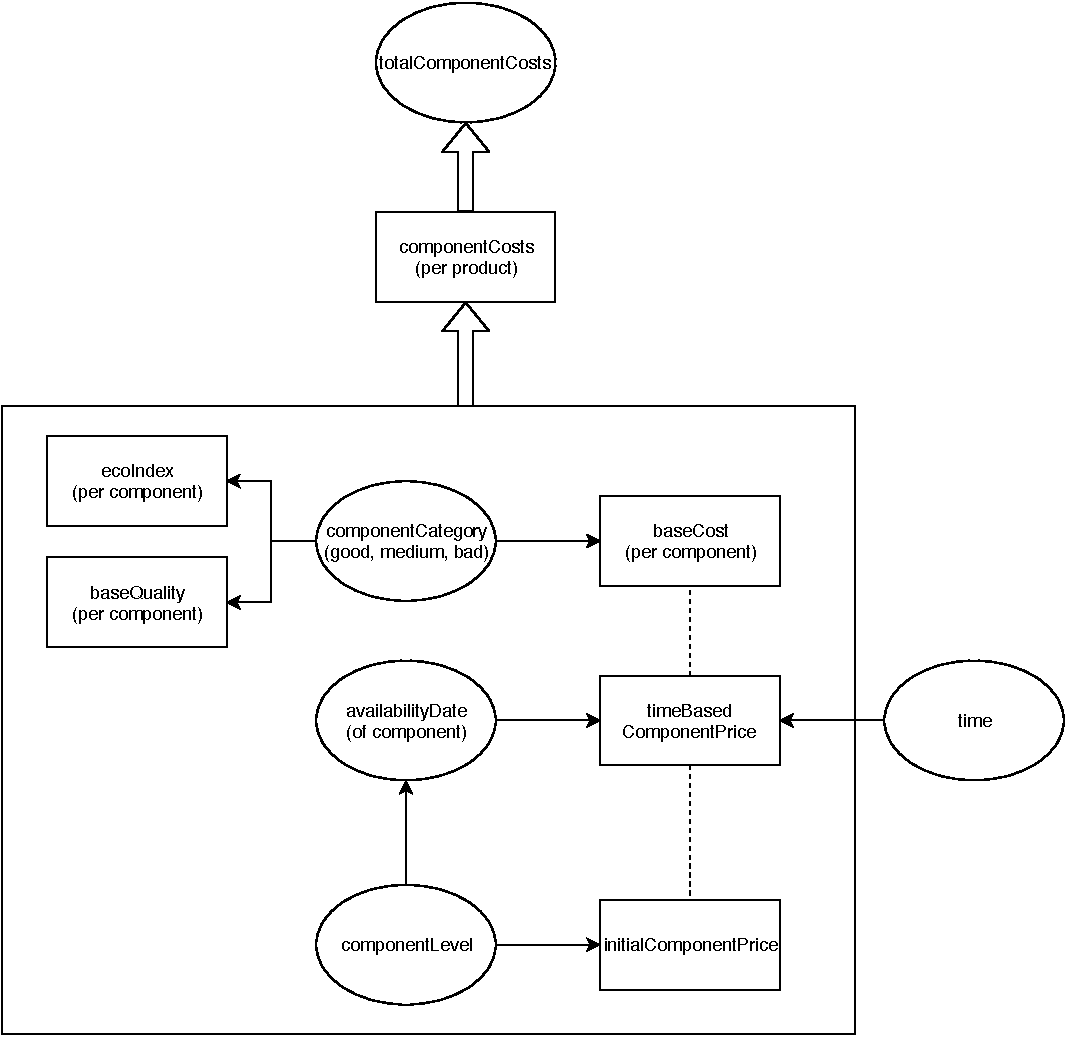
\includegraphics[width=11.5cm]{images/totalComponentCosts.pdf}
	\caption{Calculation of \textit{totalComponentCosts}}
	\label{img:totalComponentCosts}
\end{figure}

Starting from the bottom of figure \ref{img:totalComponentCosts}, the \textit{initialComponentPrice} is available for each component and depends on the \textit{componentLevel}.
The \textit{timeBasedComponentPrice} depends on the \textit{time}, on the \textit{availabilityDate} of a component, and on the \textit{initialComponentPrice}, which in turn depends on the \textit{componentLevel}.
The \textit{timeBasedComponentPrice} is dependent on the \textit{time} because we assume that a supplier produces a component in a certain level for a certain amount of time. In the first year, this is then state-of-the-art technology. However, as state-of-the-art technology rapidly become outdated and additionally new \textit{componentLevels} are released, the \textit{timeBasedComponentPrice} decreases starting from the second year on.

The \textit{timeBasedComponentPrice} is calculated by multiplying the \textit{initialComponentPrice} with the \textit{timeBasedPriceMultiplicator} (tBPM), as shown in equation \ref{Function timeBasedComponentPrice}. The \textit{timeBasedPriceMultiplicator} in turn is calculated according to the polynomic function \ref{Function timeBasedPriceMultiplicator} of fifth degree, which was interpolated from component values loosely based on historical component prices found on multiple Internet sources such as \href{https://camelcamelcamel.com}{camelcamelcamel.com}.
\begin{equation}
\label{Function timeBasedPriceMultiplicator}
\begin{aligned}
   tBPM_{c}(t_y, c) = & - 0.0001(t_y-availabilityDate_{c}+1)^5 \\
   & - 0.0112(t_y-availabilityDate_{c}+1)^4 \\
   & - 0.4239(t_y-availabilityDate_{c}+1)^3 \\
   & + 7.3219(t_y-availabilityDate_{c}+1)^2 \\
   & - 49.698(t_y-availabilityDate_{c}+1) \\
   & + 142.7889 &&
\end{aligned}   
\end{equation}
\begin{equation}
\label{Function timeBasedComponentPrice}
    tBCP_{c} (iCP, tBPM) = iCP \cdot \dfrac{tBPM}{100}
\end{equation}

\begin{figure} [H]
    \centering
	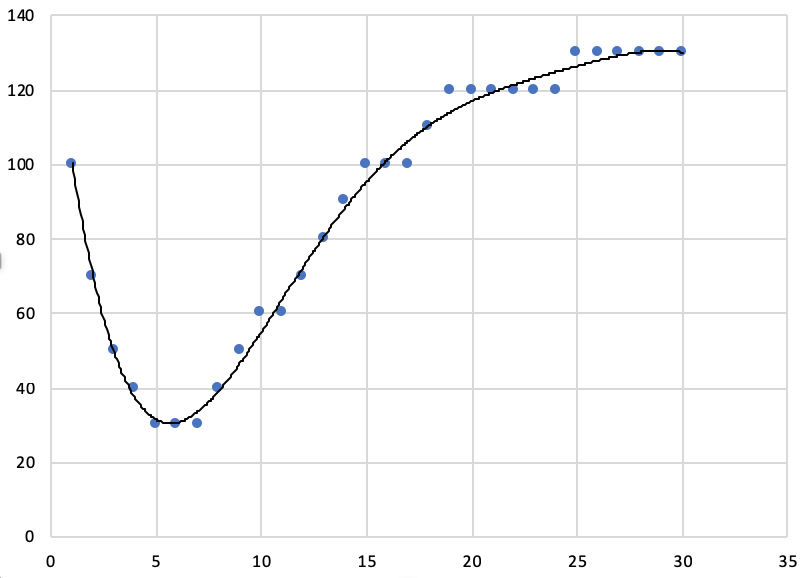
\includegraphics[width=9.5cm]{images/timeBasedComponentFunction.png}
	\caption{Function of \textit{timeBasedComponentPrice}}
	\label{img:timeBasedComponentPriceFunction}
\end{figure}
As it can be seen in picture \ref{img:timeBasedComponentPriceFunction} the \textit{timeBasedComponentPrice} decreases until the 5th year, stays stable for a short while on this reduced level, and then starts increasing again. The increase is due to the assumption that a supplier will discontinue the production of a component with a certain \textit{componentLevel} after some time because a newer level is released or available on the market. Since the supplier’s stock could be empty at this point, the component becomes a rarity. Therefore the component becomes more expensive compared to its \textit{initialComponentPrice}.\\
Afterwards, based on the \textit{timeBasedComponentPrice} and the \textit{supplierCategory} (which can either be premium, regular or cheap) a component's \textit{baseCost} is calculated. Moreover, also a component's \textit{supplierEcoIndex} and \textit{supplierQuality} depend on the \textit{supplierCategory}.\\
The \textit{componentCosts} per product can then be calculated by adding up the \textit{baseCost} of the selected components per product. All \textit{componentCosts} together then determine the \textit{totalComponentCosts} of all produced products.\\

In the following, further ideas for the procurement simulation are explained which have not yet been implemented or tested in our prototype, but which are also part of our concept.

A volume discount would allow the player to get a 10 percent discount, for example, if he buys more than 300 units of a component. We postponed this idea because our prototype does not include units in the procurement simulation yet. Currently, the player only needs to select a component and it is assumed that the desired quantity is delivered for just-in-time production. 
The aim, however, is to leave the purchase decision to the user, who would have to calculate the trade-off between the benefits of lower prices per component due to volume discounts and higher storage costs for storing all non-producible components.

\section{Production Simulation}
\label{sec:products}
Livja \\
 Production definition \\
Production process considering industry best practice \\
Measures for Production: which ones we aim to increase/ decrease \\
 Factors that affect product quality 
\begin{itemize}
\item production technology
\item employee skills
\item supplier index
\item logistics
\item warehousing (storage facilities)
\end{itemize}
Specify which factors were relevant to our simulation \\
Relate factor to the corresponding chapter, emphasize their correlation in increasing product quality, explain the 5 points Likert scale for each factor\\
Production Technology: 
\begin{itemize}
    \item Deprecated                  Scale: 1
    \item Old                         Scale: 2
    \item Good conditions             Scale: 3
    \item Purchased more than 5 years ago Scale: 4
    \item Brand new                   Scale: 5

\end{itemize}
The technology used in production starts at 5 points when all machinery is new. It lowers (-1) point over a 5 years time-span. It lowers (-2), if there is a fire, flood, hurricane.\\
This measure can be improved by:
\begin{itemize}
    \item Purchasing new machinery (level 5)
\item Maintaining \& repairing (+1)
\item Upgrading (+2)
\end{itemize}


Productivity: factors that influence it \\
Give functions, equations for measuring each of the factors that affect productivity \\
explain graph : production is dependent of the production process and the product itself 

\section{Warehouse Simulation}
Janine\ \\
% Janine \\
\begin{itemize}
    \item All produced products go directly into the warehouse but it only costs if they are not sold / delivered at the same day they are produced.
    \item For each product in the warehouse at the end of the day (after all packages are delivered according the demand) the company has to pay
    \item If the warehouse is full, it shouldn't’t be possible to produce more products. That means production is limited to the storage capacity! 
    \item Storage capacity is shared between components and products. To make it a bit more realistic: components need 1/2 unit and products 1 unit
    \item number of products in the warehouse forms the basis for the number of products that can be sold
    \item Characteristics 
    \begin{itemize}
        \item can be build / bought or rented
        \item linear depreciation over 25 years, building losses every year AC/25 on value 
        \item capacity of 5000 units
    \end{itemize}
    \item Cost 
    \begin{itemize}
        \item building-costs (one time) | rental cost (monthly)
        \item maintenance costs (yearly or monthly) 
        \item Daily costs for storage = number units * storing cost per unit per day
    \end{itemize}
\end{itemize}

\section{Logistic and Support Simulation}
Janine\ \\
\subsection{Logistic}
% The delivery of the products always takes place at the end of the day directly from the warehouse. Basically there are three ways to manage the logistic of the company: 
\begin{itemize}
    \item The company has its own logistics fleet
    \item The company has outsourced the logistics to an external partner
    \item The company simply sends products by mail
\end{itemize}

The player can combine these variants in the way he considers best for his company.  Basically, there are four logical approaches:
\begin{enumerate}
    \item The player decides to send all his products by post 
    \item The player decides to completely outsource the logistics and signs a contract with an external logistics partner
    \item The player exclusively employs his own logistics fleet and ships products that exceed his delivery capacity at high cost by post
    \item The player has his own fleet and delivers products which exceed his capacity by an external logistics partner
\end{enumerate}
	
In the following sections, the functionality of the individual variants and the costs incurred are explained in detail.

\subsubsection{Internal logistic fleet}
The internal logistics fleet consists of purchased trucks and the company's logistics employees. The quality of the company's own logistics is calculated on the basis of their characteristics and motivation.

Every truck has certain characteristics, these consist of:
\begin{itemize}
    \item A capacity of products that can be transported, this is the same for all trucks and amounts to 1000 packages. For reasons of simplification, we do not distinguish the size of individual products.  Each product is equivalent to one package. 
    \item An environmental index that expresses how environmentally friendly the vehicle is.
    \item A quality index that expresses the quality of the transport.
    \item A purchase price that depends on the quality and environmental friendliness of the truck.
    \item Monthly maintenance costs corresponding to ...\% of the initial purchase price divided by 12 months (REFERENCE)
    \item And a depreciation rate that is linear and amounts to 9 years for each truck (REFERENCE) 
\end{itemize}

----

Internal logistic:
\begin{itemize}
    \item The capacity of the logistics fleet is measured by the number of trucks
    \item If the demand for products is higher than the inventory, all products are sold from the warehouse. That means the inventory represents the maximum sales quantity for a product
    \item If the demand for a product is lower than the inventory, only the demanded quantity is sold and thus delivered. The remaining products stay in the warehouse and cause storage costs 
    \item Trucks
    \begin{itemize}
        \item Capacity = 1000 products  
        \item purchase price = tbd 
        \item maintenance cost (yearly or monthly) = tbd
        \item eco index (EF) = [20,40,60,80,100]
        \item quality index (QF) = [20,40,60,80,100]
        \item Logistic employees: Quality of work (QWLE)
        \item Depreciation 
        \begin{itemize}
            \item linear over 9 years
            \item = aquicion cost / 9 
        \end{itemize}
        \item Fleet index (FI) = EF*0,2 + QF*0,8
        \item  = FI*0,6 + QWLE*0,4
        \item Internal logistic index (ILI)
        \begin{itemize}
            \item If $QWLE \leq \ $40: (FI*0,5 + QWLE*0,5)
            \item Else: (FI*0,6 + QWLE*0,4)
        \end{itemize}
    \end{itemize}
    \item Delivery Cost:
    \begin{itemize}
        \item number of products = deliver capacity: deliver costs  = (number of products / 1000) * cost per delivery
        \item number of products < deliver capacity: delivery cost = round up to the next int (number of products / 1000) * cost per delivery
        \item number of products > deliver capacity: delivery cost = number trucks * cost per delivery + cost delivery external (-> see cost external logistic partner) 
        \item if no external logistic partner is hired, the delivery of one product costs -tbd
    \end{itemize}
\end{itemize}

External logistic partner:
\begin{itemize}
    \item The player is able to fire the actual partner and hire a new one. Only one logistic partner at the same time should be possible. (can be hired in the job market)
    \item If an external partner is hired own trucks are not needed but can be
    \item Characteristics of the partners:
    \begin{itemize}
        \item Quality (QLP) = [20,40,60,80,100]
        \item Eco-Index (ELP)= [20,40,60,80,100]
        \item Reliability (RLP) = [20,40,60,80,100]
    \end{itemize}
    \item Beyond a certain limit of reliability, this characteristic of an external partner has a greater impact on the external logistic index: $Reliability \leq \ $40
    \item External logistic index (ELI)
    \begin{itemize}
        \item If $RLP \leq \ $40: (RLP*0,5 + 0,5*(QLP*0,8 + ELP*0,2))
        \item Else: (RLP*0,4 + 0,6*(QLP*0,8 + ELP*0,2))
    \end{itemize}
    \item Cost of an external logistic partner:
    \begin{itemize}
        \item cost per delivery of one package 
        \item contractually agreed fixed costs (yearly or monthly)
        \item cost delivery external = (number of products - number trucks * 1000) * cost per delivery of one package (external)
    \end{itemize}
\end{itemize}

logistic index (LI):
\begin{itemize}
\item (ELI * number packages delivered external + ILI * number packages delivered internal) / number all packages delivered 
\end{itemize}

\subsection{Product Support}
% Product Support:
\begin{itemize}
\item only possible with sales employees 
\item support infrastructure cost: initial cost + yearly maintenance cost  
\item Based on the support type, the quality o work (QWSE) and the job satisfaction (JSSE) of the sales employees
\item Types and indexes (STI)
\begin{itemize}
\item No product service (0)
\item online self service = 5
\item online support = 25
\item telephone support = 30  
\item store support = 40
\item All four (100)
\end{itemize}
\item Employee Index Sales (EIS) = JSSE*0,4 + QWSE*0,6
\item Support type index (STI) = Sum Indexes offered support types
\item Product support index (PSI) 
\begin{itemize}
\item If $EIS \leq \ $50: (0,4*EIS + STI*0,6)
\item Else: (0,4*EIS + STI*0,6)
\end{itemize}
\end{itemize}

Overall support (OS)
\begin{itemize}
\item If LI $LI \leq \ $40: (LI*0,5 + PSI*0,5)
\item ElseIf $LI \leq \ $50: (LI*0,6 + PSI*0,4)
\item Else: (LI*0,7 + PSI*0,3)
\end{itemize}

\section{Marketing Simulation}
Janine\ \\
\subsection{Market Research}
% \gls{cs} %Customer Satisfaction from glossary
\subsubsection{Price Sensitive Research}
    \begin{itemize}
        \item Provides a price sensitive analysis for a specific product
        \item The research shows the results for 9 price levels around the reference price (input), the price levels are from -20\% to +20\% in 5\% steps
        \item more than the reference value: x = ((100 * new value) / ref value) - 100
        \item less than the reference value: x = ((1 - (new value / ref value)) / 100
        \item Output includes: 
        \begin{itemize}
            \item all the values are calculated based on the actual values and the defined market price, changes are calculated based on the reference market price 
            market price
            \item margin, sales number, sales volume, total cost, market share, margin change, market share change
        \end{itemize}
        \end{itemize}
       
       \begin{table}[ht]
        \centering
        \begin{tabular}{|l|r|r|r|r|r|r|r|r|r|}
        \hline
        key figures             & -20\% & -15\% & -10\% & -5\%  & 0\%   & +5\%  & +10\% & +15\%   \\
        market price            &       &       &       &       &       &       &       &         \\
        product costs           &       &       &       &       &       &       &       &         \\
        margin                  &       &       &       &       &       &       &       &         \\
        sales number            &       &       &       &       &       &       &       &         \\
        sales volume            &       &       &       &       &       &       &       &         \\
        market share            &       &       &       &       &       &       &       &         \\
        margin change           &       &       &       &       &       &       &       &         \\
        market share change     &       &       &       &       &       &       &       &         \\
        net change              &       &       &       &       &       &       &       &         \\
        \hline
        \end{tabular}
        \caption{Structure price sensitive research}
        \label{MR_price_sensitive}
        \end{table}

\subsubsection{Customer Satisfaction Research}
    \begin{itemize}
        \item company at all (last four quarters): Calculation of the customer satisfaction for the last four quarters 
        \item specific product (last four quarters): Calculation of the customer satisfaction for the specific product for the last four quarters 
    \end{itemize}
    
    \begin{table}[ht]
    \centering
    \begin{tabular}{|l|r|r|r|r|}
    \hline
                & quarter 1   & quarter 2  & quarter 3 & quarter 4 \\
    product 1   &             &            &           &           \\
    product 1   &             &            &           &           \\
    product 1   &             &            &           &           \\
    ...         &             &            &           &           \\
    total       & average     & average    & average   & average   \\
    \hline
    \end{tabular}
    \caption{Structure customer satisfaction research}
    \label{MR_customer_satisfaction}
    \end{table}
    
\subsubsection{Market Statistic Research}
    \begin{itemize}
        \item overall company, product level
        \item provides a variety of market information: 
        \item Costs: fix price for external and internal survey
        \item Includes: product price, market share, sales numbers, product quality, service quality 
    \end{itemize}
    
    \begin{table}[ht]
    \centering
    \begin{tabular}{|l|r|r|r|r|}
    \hline
                            & product 1   & product 2  & product 3 & ...       \\
    product price           &             &            &           &           \\
    market share            &             &            &           &           \\
    sales numbers           &             &            &           &           \\
    product quality         &             &            &           &           \\
    service quality         &             &            &           &           \\
    customer satisfaction   &             &            &           &           \\
    \hline
    \end{tabular}
    \caption{Structure market statistic research}
    \label{MR_market_statistic}
    \end{table}

\subsection{Lobbyist}
% \subsection{Lobbyist} \label{lobbyist_simulation}
%Janine

If the company is in contact with a lobbyist, he tries to mitigate negative government decisions on the company. For its services the lobbyist demands a monthly compensation \textit{price}. The effect of the lobbyist is reflected by the \textit{taxRate}. 

Only one lobbyist can be assigned at a time, if the player wishes to hire another lobbyist, he must first fire the current one. Each lobbyist has a \textit{type}, a \textit{price} and a \textit{taxRate}. The \textit{type} determines how influential the lobbyist is, more precisely how high the \textit{taxRate} is due to his influence. The player can choose between four different lobbyists: Mayor, Worker’s Union Leader, Congressman and Senator. The Senator is the most influential but also the most expensive lobbyist. Table \ref{influence_lobbyist} shows the relationship between \textit{type}, \textit{taxRate} and \textit{price}. 

\begin{table}[ht]
\centering
\begin{tabular}{|l|r|r|}
\hline
Type                    & taxRate   & price in cc \\ \hline
Mayor                   & 18\%      & 1000     \\
Worker's Union Leader   & 16\%      & 1000     \\
Congressman             & 13\%      & 5000     \\
Senator                 & 10\%      & 10000     \\
\hline
\end{tabular}
\caption{Influence and price lobbyist}
\label{influence_lobbyist}
\end{table}

In order to find out which lobbyist is the most rewarding one for the company, the player must calculate the amount of the tax reduction and compare it with the \textit{price} incurred by the lobbyist.
 



 






\subsection{Management Consultancy}
% If the company contacts a management consultancy, they try to investigate possible optimization points and report them to the player. (ToDo: Whats the goal of the consultancy -> optimize customer satisfaction?) 



\section{Customer Simulation}
\label{sec:customsim}
Janine, Maike \\
Most common types of customer needs regarding products and the main levels of customer requirements: Functionality, price, design, reliability/availability/durability, performance, safety and sustainability
\\
The customer simulation is a weighted combination of the product price and the customer satisfaction. 
That means that customer satisfaction and price are the two key indicators for the buying decision of the customers. The buying decision determines to what extent the customers are willing to buy a product. 
For example: Buying Decision (Price, Customer Satisfaction) = 0,6 * Price + 0,4 * Customer Satisfaction
\\
 Levels of customer requirements: Must haves, satisfiers and delighters. Must haves are the bare minimum requirements expected of customers. The customers do not show exceptional appreciation for the must haves, but if they are not met, the customer will show dissatisfaction. Satisfiers are the requirements that the customer expressly wishes. If you offer better or more of these satisfiers, then the customers will appreciate it more and be more satisfied. Delighters are the extras or the add-ons. The lack of these characteristics will not make the customer dissatisfied but adding these would greatly increase the customer's satisfaction. In our game, realized these three levels of customer requirements in the context of our product components. If the user chooses newer, better components for producing his / her product, then specific satisfiers or delighters are met, depending on how good the chosen components are.
 \\
 Main categories of customer satisfaction that are necessary for our game: \\
- Satisfaction with the support quality, based on \\
    o Satisfaction with the support quality \\
    o Satisfaction with the support \\
- Satisfaction with the product quality, based on \\
    o Satisfaction with the product quality \\
    o Satisfaction with the design of the product \\ 
- Satisfaction with the company image \\
\\

Calculation
\begin{itemize}
    \item Overall Product Quality (OPQ)
    \item Overall support (OS) reference calculation in support (ToDo)
    \item Company branding (CB) = 0,9*Company Image + 0,1*Job Satisfaction
    \item Employer branding (EB) 
    \item Customer Satisfaction (CS)
    \begin{itemize}
    \item If $OPQ \leq \ $40: (0,75*OPQ + 0,1*OS + 0,1*CB + 0,05*EB )
    \item ElseIf $OPQ \leq \ $60: (0,65*OPQ + 0,2*OS + 0,1*CB + 0,05*EB)
    \item Else: (0,55*OPQ + 0,3*OS + 0,1*CB + 0,05*EB)
    \end{itemize}
\end{itemize}

\section{Competitor Simulation}
Steffen

Janine \\
Demand simulation: 
\begin{itemize}
\item How much products are sold depends on the Customer Satisfaction and also the sum of the component prices in the current year. We assume the potential customers use as baseline a product with the most recent components. 
\item The customer satisfaction influences how much the customers are willing to pay for the product 
\item The component prices are the basis for the price were 100\% are sold. This is defined for the customer satisfaction to be between 50 and 40
\begin{itemize}
\item CS >= 80: component price * 1,2 
\item 80 \textgreater $CS \geq \ $60: component price * 1,1
\item 60 \textgreater $CS \geq $50: component price * 1,05
\item 50 \textgreater $CS \geq $40: component price * 1
\item 40 \textgreater $CS \geq $20: component price * 0,9
\item CS \textless 20: component price * 0,8
\end{itemize}
\item In order to determine what percentage of the offered products will be sold (y) the chosen retail price divided by the base price in the current year will be used as x in the following formula.
\begin{equation}
%y = 167.905104 * \E^{ -2.990914872 * 10^{ -1 } * x^{ 2 }}
\end{equation}
\begin{itemize}
    \item if the result is \textgreater 100; demand = 100\%
    \item if the result is \textless 0; demand = 0\%
\end{itemize}
\end{itemize}

\section{Linkages \& Interdependencies}
\label{sec:link}
Overall Graph

\section{Example Flowboard}
A flowboard is the best way to document a game’s structure. The term is derived
from a flowchart and a storyboard. Storyboards are a linear series of pictures
used by filmmakers to plan a set of shots. Flowcharts are diagrams used
by programmers for documenting an algorithm. A flowboard combines these
two ideas. Each picture is a sketch or a mockup of the screen, in one specific
gameplay mode or menu. The pictures are connected via arrows that indicate
under what circumstances the transition takes place. (1, p. 57; 3.) The flowboard
does not necessarily need pictures in it to work. A simpler approach (Figure
2) might even be better in some cases.

\section{External events}
This section deals with the influence of events that happen during the course of the game. Companies have to deal with influencing factors which are neither planned nor foreseeable\cite{Campbell}. This section refers to 'external' events as they are out of the players explicit and obvious control. Actions taken may still have an influence on an event's probability to happen, but this is invisible for the player. From a location point of view events can take place inside the company, for example strikes, or outside like rising taxes. Punishment for mistakes is common, but the player may also be rewarded when outstanding performance is present.  
There are 19 distinct events divided into 5 categories and acting as counterparts to the game features. In addition, they reflect different areas of of the company's business: 

\begin{itemize}
\item Production and Market events map to the production and procurement simulation. 
\item Money and Taxes. intervene with content of the finance simulation.  
\item Employees covers one event (strikes) which deals with the HR simulation.
\item Natural Disasters have an internal source for gaming purposes, but come from outside of the company. 
\item Government and Politics are a mostly invisible force that acts in the game. They are not visible to the player, but the impact is significant. 
\end{itemize}

Events are usually cross-functional. This means that the trigger of an event in a specific category comes from another one. This is also the case for the outcome of events. The categorization itself orientates on the nature of the event.

Characteristics of the events
\begin{itemize}
\item Random vs. Conditional probability
\item Rising Probability vs. Certain occurrence
\item Threshold applicable: yes / no
\item Impact on an Game Mechanic: yes / no
\end{itemize}
The decision which event should get which characteristic was based on multiple aspects. In general, a business simulation intends to reflect the real-world which is also applicable for events. Their nature and likeliness to happen are to be transferred to the game environment. But there are aspects which are contradictory to this intend. Empirical evidence for the probability of events might be rare or the probability is so low that they would happen almost never throughout the game. Events having such an impact that they lead to a Game-Over must not happen in an early state and frustrate the player. In the end gaming should be fun too, not only replaying the real-world. Reflecting the latter is also limited as a simulation can never cover every 'live' aspect. As a result of these considerations, a probability can distort from its real-world example. If suitable, an event can even have a complete random occurrence providing a more challenging game experience to the player. This is the case for 5 events. 



Adapting real-world examples in most cases, all events have in common that they have a significant impact on an indicator of the game mechanics. Some events are exaggerated compared to real-world examples. 


\begin{landscape}
\begin{table}[]
%{
\fontsize{7}{8} \selectfont
\begin{tabular}{|l|l|l|l|l|l|l|l|l|}
\hline
 & \textbf{External Event} & \textbf{\begin{tabular}[c]{@{}l@{}}Random / \\ Conditional\end{tabular}} & \textbf{\begin{tabular}[c]{@{}l@{}}Influencing \\ Indicators\end{tabular}} & \textbf{\begin{tabular}[c]{@{}l@{}}Starting \\ Threshold\end{tabular}} & \textbf{\begin{tabular}[c]{@{}l@{}}Probability or\\ Preconditions\end{tabular}} & \textbf{\begin{tabular}[c]{@{}l@{}}Final \\ Threshold\end{tabular}} & \textbf{Impact on} & \textbf{Remarks} \\ \hline
\textbf{} & \textbf{Production and Market:} & \textbf{} & \textbf{} & \textbf{} & \textbf{} & \textbf{} & \textbf{} &  \\ \hline
1 & \begin{tabular}[c]{@{}l@{}}Production Problems \\ PopUp\end{tabular} & Conditional & \begin{tabular}[c]{@{}l@{}}Product\\ Quality\end{tabular} & 0,3 & (-1*Product Quality+2) & 0 & n/a & Decreasing Function \\ \hline
2 & \begin{tabular}[c]{@{}l@{}}New technology \\ increases Quality\end{tabular} & Conditional & \begin{tabular}[c]{@{}l@{}}Product \\ Quality\end{tabular} &  &  &  & Customer Satisfaction & \begin{tabular}[c]{@{}l@{}}Boosts Customer \\ Satisfaction for 20 cycles\end{tabular} \\ \hline
3 & \begin{tabular}[c]{@{}l@{}}Company Aqcuistion \\ possibility offered\end{tabular} & Conditional & \begin{tabular}[c]{@{}l@{}}Constant \\ Increasing \\ Revenue\end{tabular} & n/a & \begin{tabular}[c]{@{}l@{}}Revenue increases\\ 25\% per year \\ over 5 years\end{tabular} &  & \begin{tabular}[c]{@{}l@{}}Indicators of \\ Acquisition integrated\end{tabular} & \begin{tabular}[c]{@{}l@{}}Acquistion costs xy, \\  minigame possible\end{tabular} \\ \hline
4 & \begin{tabular}[c]{@{}l@{}}Large company \\ overtakes market share\end{tabular} & Random & n/a &  & 0,05 &  & Revenue & \begin{tabular}[c]{@{}l@{}}Only possibe if revenue \\ above xx CapCoins\end{tabular} \\ \hline
5 & \begin{tabular}[c]{@{}l@{}}Company Brand \\ reputation plunges\end{tabular} & Conditional & \begin{tabular}[c]{@{}l@{}}Customer \\ Satisfaction\end{tabular} & n/a & \begin{tabular}[c]{@{}l@{}}Customer satisfaction \\ below threshold of XY\end{tabular} & n/a & Demand &  \\ \hline
6 & \begin{tabular}[c]{@{}l@{}}Computer virus \\ attacks\end{tabular} & Random & n/a & n/a & 0,1 & n/a & \begin{tabular}[c]{@{}l@{}}Productivity and\\ Reputation\end{tabular} & After Year 2000 \\ \hline
\textbf{} & \textbf{Finance and Taxes:} & \textbf{} & \textbf{} & \textbf{} & \textbf{} & \textbf{} & \textbf{} & {\color[HTML]{FE0000} } \\ \hline
7 & \begin{tabular}[c]{@{}l@{}}Tax Changes lead to \\ higher or less rates\end{tabular} & Random & n/a & n/a & -2 to 5 percent &  &  & In-/Decrease over time \\ \hline
8 & Stricter Eco Laws & Conditional & \begin{tabular}[c]{@{}l@{}}Eco \\ Index\end{tabular} & 2 & 0.12 * Eco Index \textasciicircum 1.3 & 5 & \begin{tabular}[c]{@{}l@{}}Financial Fine or \\ Game Over\end{tabular} & Shutdown by Government \\ \hline
9 & Inflation changes & Random & n/a & n/a & \begin{tabular}[c]{@{}l@{}}0 - 2 \% \\ (random)\end{tabular} & n/a &  & Example Germany \\ \hline
10 & \begin{tabular}[c]{@{}l@{}}Stealing inside of\\ the company\end{tabular} & Conditional & \begin{tabular}[c]{@{}l@{}}Job \\ Satisfaction\end{tabular} & 50\% & \begin{tabular}[c]{@{}l@{}}-4 * Job\\ Satisfaction + 2\end{tabular} & 25\% & Revenue & \begin{tabular}[c]{@{}l@{}}Financial decrease even \\ if sales high and cost \\ low (Incosistency)\end{tabular} \\ \hline
\textbf{} & \textbf{Employees:} & \textbf{} & \textbf{} & \textbf{} & \textbf{} & \textbf{} & \textbf{} &  \\ \hline
11 & Strikes and union fightings & Conditional & Salary &  & Scaling to be defined &  & \begin{tabular}[c]{@{}l@{}}Production \\ Performance\end{tabular} & \begin{tabular}[c]{@{}l@{}}Only ends when \\ salaries are risen\end{tabular} \\ \hline
\textbf{} & \textbf{Natural Disasters:} & \textbf{} & \textbf{} & \textbf{} & \textbf{} & \textbf{} & \textbf{} &  \\ \hline
12 & \begin{tabular}[c]{@{}l@{}}Flu goes around \\ causing Ill employees\end{tabular} & Random & n/a & n/a & 0,2 & n/a & \begin{tabular}[c]{@{}l@{}}Productivity \\ Decrease of 10\%\end{tabular} & \begin{tabular}[c]{@{}l@{}}Temporary impact vanishes\\ after 100 Game Cycles\end{tabular} \\ \hline
13 & \begin{tabular}[c]{@{}l@{}}Hurricanes, tornados, \\ earthquakes\end{tabular} & Conditional & \begin{tabular}[c]{@{}l@{}}Eco \\ Index\end{tabular} & 2 & 0.12 * Eco Index \textasciicircum 1.3 & 5 &  &  \\ \hline
14 & \begin{tabular}[c]{@{}l@{}}Fire / Flooding in \\ warehouse\end{tabular} & Conditional & Inventory & \begin{tabular}[c]{@{}l@{}}Warehouses \\ at 80\%\end{tabular} & Game Cycles *0,001 & \begin{tabular}[c]{@{}l@{}}100 Game \\ Cylces\end{tabular} & Inventory & \begin{tabular}[c]{@{}l@{}}Only if warehouse\\ at or over 80\% full\end{tabular} \\ \hline
\textbf{} & \textbf{Government and Politics:} & \textbf{} & \textbf{} & \textbf{} & \textbf{} & \textbf{} & \textbf{} &  \\ \hline
15 & \begin{tabular}[c]{@{}l@{}}Problems with customs \\ at the harbour\end{tabular} & Conditional & \begin{tabular}[c]{@{}l@{}}Supplier \\ quality\end{tabular} &  & Future work &  &  &  \\ \hline
16 & Change of power & Random & n/a & n/a & 0,2 &  & Tax rate & Most once the whole game \\ \hline
17 & Anonymous bomb threats & Conditional &  &  &  &  &  &  \\ \hline
18 & \begin{tabular}[c]{@{}l@{}}Blocked roads \\ beacause of riots\end{tabular} & Conditional & Company Image &  & Future work &  &  &  \\ \hline
19 & \begin{tabular}[c]{@{}l@{}}Tensions between our \\ country and other countries\end{tabular} & Conditional & \begin{tabular}[c]{@{}l@{}}Change \\ of Power\end{tabular} & n/a & n/a & n/a & n/a & Future Work \\ \hline
\end{tabular}
    \caption{External events}
    \label{events_list}
\end{table}
\end{landscape}

The event list can be further extended when more game features are developed. Some events are proposed as ideas as the features they are based on are not conceptualized yet.
\section{Prototype implementation}
Steffen\\
Mechanics, how we did testing\\
Testing in each section

\chapter{Marketing Proposals}
Philipp\\
\label{cha:exp}
\label{sec:setting}
How to sell to company


\chapter{Conclusion}
\label{cha:conclusion}


\section{Summary}
\label{sec:sum}

\section{Future Work}
\label{sec:future}
Idea List\\
Mobile device integration
Future timeline
AR, VR support
Multiple countries that will enable online multi-players
3rd phase of the game corporate utopia
\bibliographystyle{plain}
\bibliography{thesis-ref}


\appendix

\chapter{Appendix}
\label{cha:appendix-a}

\newpage


\pagestyle{empty}


\end{document}
